\documentclass[12pt]{article}
\usepackage[margin=1in]{geometry}
\usepackage[spanish,es-lcroman]{babel}
\usepackage{amsmath,amsthm,amssymb,amsfonts}
\usepackage{graphicx}

\newcommand{\Cp}{\texttt{C+-}}
\newcommand{\C}{\texttt{C}}
\newcommand{\Cpp}{\texttt{C++}}

\newenvironment{problem}[2][Problem]{\begin{trivlist}
\item[\hskip \labelsep {\bfseries #1}\hskip \labelsep {\bfseries #2.}]}{\end{trivlist}}
%If you want to title your bold things something different just make another thing exactly like this but replace "problem" with the name of the thing you want, like theorem or lemma or whatever


\begin{document}

%\renewcommand{\qedsymbol}{\filledbox}
%Good resources for looking up how to do stuff:
%Binary operators: http://www.access2science.com/latex/Binary.html
%General help: http://en.wikibooks.org/wiki/LaTeX/Mathematics
%Or just google stuff

\title{Reporte 2. Analisador semántico para el Lenguaje C+-}
\author{Mat\'ias Greco, Javier Reyes}
\date{9 de Noviembre, 2018}
\maketitle

\section*{Introducci\'on}
El presente reporte explica el trabajo realizado para el desarrollo de un anailzador sem\'antico para el lenguaje de programaci\'on \Cp.

El lenguaje \texttt{C+-} corresponde a un subconjunto del lenguaje \C, con la adici\'on de algunas caracter\'isticas de \Cpp, como la posibilidad de definir una funci\'on con paso por valor o paso por referencia.

El an\'alisis  ' l\'exico y sint\'actico de este lenguaje de programación fue desarrollado previamente, obtenido un arbol sintáctico abstracto (AST) el cual se recorre nodo a nodo. Dicho analizador fue desarrollado en la herramienta ANTLR4 (ANother Tool for Language Recognition) con lenguaje de salida \Cpp. 

El analisador sem\'antico fue desarrollado en el lenguaje de programación Python y su salida es una tabla de simbolos en la cual se encuentran todos los simbolos necesarios para desarrollar el an\'alisis sem\'antico correspondiente, y donde cada subarbol representa un \'ambito dentro del programa.

El repositorio del proyecto está disponible en github\footnote{https://github.com/matgreco/Cmm-Compiler}.


\section*{Caracter\'isticas del lenguaje}

El lenguaje \texttt{C+-} incluye las siguientes caracter\'isticas, propias del standard \texttt{C89}
\begin{itemize}
    \item Funciones.
    \item Declaraciones.
    \item Asignaciones.
    \item Expresiones l\'ogicas y de operaciones.
    \item If.
    \item Switch (case y default).
    \item While.
    \item For.
    \item Do While.
    \item Struct.
\end{itemize}

Algunas caracter\'isticas interesantes incluidas:
\begin{itemize}
    \item Comma expression
\end{itemize}

\subsection*{Caracter\'iticas no incluidas}
\begin{itemize}
    \item Macros:

    No se incluy\'o debido a que complica todo el proceso. Requerir\'ia una precompilaci\'on y la capacidad de incluir otros archivos mediante enlazado.
    \item Punteros:

    No se incluy\'o debido a que complica la gram\'atica, por la aparici\'on de una infinidad de tipos distintos (del estilo \texttt{int***}). Tambi\'en requiere una administraci\'on de memoria que escapa de nuestro objetivo principal.

    \item Typedef:

    No se incluy\'o debido a que complica la definici\'on de la gram\'atica. Eso permitir\'ia utilizar una expresi\'on de tipo \texttt{VAR} como una definici\'on de tipo. Al no incluirlo, el lenguaje no pierde capacidades, ya que una estructura personalizada \texttt{S} tiene tipo \texttt{struct S}.
\end{itemize}


\subsection*{Representací\'on de la tabla de s\'imbolos}
En el proceso de compilaci\'on, luego de la generaci\'on del AST, es necesario conocer una serie de nombres y cierta informaci\'on de para realizar el proceso de an\'alisis sem\'antico. Para esto, los compiladores prefieren almacenar y luego recuperar la informaci\'on obtenida en las lineas anteriores del programa en vez de buscarlas o recomputarlas nuevamente. Para esto existe la tabla de simbolos, que en general corresponde a una representaci\'on de un arbol cuyos son \'ambitos que almacenan tablas de hash.

\centerline{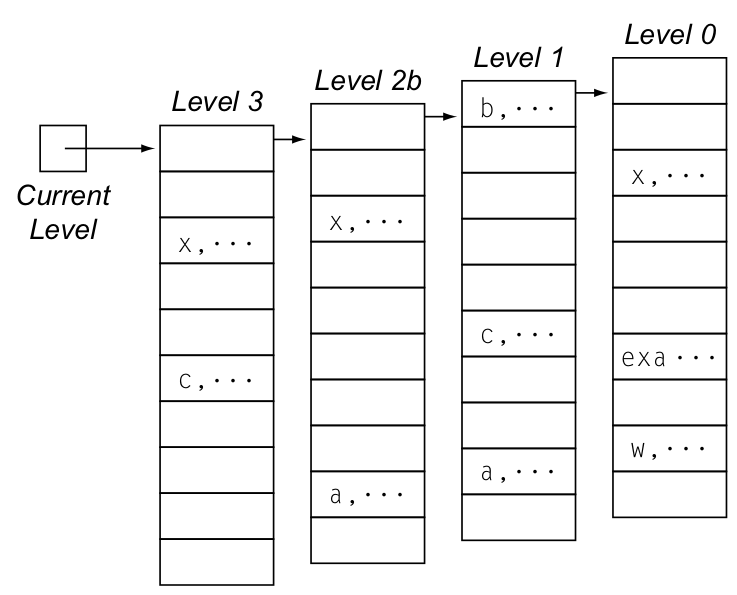
\includegraphics[trim={0 9cm 0 0},scale=0.45]{SYmTabex.png}}
\centerline{Figura 1: Representaci\'on de una tabla de simbolos. Fuente: (Cooper, 2012)}

Cada tabla de hash representa la informaci\'on contenida dentro de un \'ambito, y dicha informaci\'on solo ser\'a accesible desde los nodos sucesores. La ra\'iz del arbol representa el \'ambito global. 

Para esta implementaci\'on se utiliz\'o la biblioteca de Python AnyTree y la estructura de datos diccionario.


\subsection*{Reglas sem\'anticas}

La regla sem\'antica principal es que cada par\'entesis encargado de iniciar un \'ambito, generar\'a un nuevo nodo dentro del \'arbol de la tabla de s\'imbolos y al momento de cerrar el \'ambito volver\'a a su nodo anterior.

Cada nodo corresponde a un diccionario que en su \'indice contiene el nombre del s\'imbolo y almacena algunos datos propios de la definici\'on encontrada en el form\'ato de una estructura llamad\'a \texttt{simbol}. 

La estructura \texttt{simbol} contiene los siguientes atributos:

\begin{itemize}
    \item  \textbf{Stype:} Define el tipo de s\'imbolo encontrado. Ejemplo: 'funci\'on', 'struct', 'variable', 'valor'.
    \item  \textbf{Name:} Define el nombre del simbolo encontrado. Este es coincidente con el \'indice con el cual se agrega a la tabla de s\'imbolos.
    \item  \textbf{Vtype:} Define el tipo de dato correspondiente. En el caso de una funci\'on contendr\'a el tipo que retorna, en el caso de una definici\'on el tipo del cual es propia la variable. 
    \item  \textbf{Info:} Contiene antecedentes adicionales del s\'imbolo. Por ejemplo, el n\'umero de argumentos de una funci\'on o el numero de datos miembro una estructura. 
    \item  \textbf{Line:} Corresponde a la l\'inea en la cual fue encontrado el s\'imbolo. Ser\'a \'util para retornar mensajes de error como: "Redeclaraci\'on de la variable X, ya fue definida en la l\'inea Y". 

Una particularidad de nuestro analisador sem\'antico es que a la tabla de s\'imbolos tambien agrega los ciclos y las funciones como un nodo del \'arbol. Esto permite detectar el tipo de dato a retornar por la funci\'on o si el \'ambito corresponde a un ciclo, con la intenci\'on de hacer verificaciones como la instrucci\'on continue o break est\'en dentro de un ciclo, o si una funci\'on de tipo void tiene un valor en su instrucci\'on return.

Ejemplo de una tabla de s\'imbolos con ciclos.

\begin{verbatim}
int main(){

    while(1){
        {
            break;
            while(0){
                continue;
            }
        }
    }

    return 0;
}
\end{verbatim}

Este programa construye la siguiente tabla de s\'imbolos:
\begin{verbatim}
 {'main': (int)}
└──  {'%return': 'int'}
    └──  {'%loop': 'while'}
                └──  {'%loop': 'while'}
\end{verbatim}







**************** APENDICEE
\section*{APENDICE}

\subsection*{Definiciones l\'exicas}

La definici\'on de los componentes l\'exicos del lenguaje \texttt{C+-} es similar al lenguaje \C, y se define de la siguiente forma:
\begin{itemize}
    \item \textbf{Keywords:} \texttt{int}, \texttt{char}, \texttt{double}, \texttt{float}, \texttt{long}, \texttt{short}, \texttt{unsigned}, \texttt{sizeof}, \texttt{if}, \texttt{else}, \texttt{while}, \texttt{for}, \texttt{break}, \texttt{continue}, \texttt{true}, \texttt{false}, \texttt{struct}, \texttt{void}, \texttt{return}, \texttt{switch}, \texttt{case}, \texttt{default}, \texttt{do}. Tienen el mismo uso que en \C.
    \item \textbf{Identificadores:} Puede componerse de letras, n\'umeros y guiones bajos, pero no pueden empezar con un n\'umero.
    \item \textbf{Valores constantes:} Pueden ser n\'umeros enteros con o sin signo (expresables en base 8, 10 y 16), n\'umeros de punto flotante, caracteres y strings.
    \item \textbf{Operadores aritm\'eticos:} \texttt{+} para suma, \texttt{-} para resta, \texttt{*} para multiplicaci\'on \texttt{/} para divisi\'on y \texttt{\%} para el resto de la divisi\'on.
    \item \textbf{Operadores de comparaci\'on:} \texttt{==}, \texttt{!=}, \texttt{<=}, \texttt{>=}, \texttt{<}, \texttt{>}.
    \item \textbf{Operadores unarios:} \texttt{++}, \texttt{--}, \texttt{+}, \texttt{-}, \texttt{!}, $\mathtt\sim$.
    \item \textbf{Operadores de shift:} \texttt{<{}<}, \texttt{>{}>}.
    \item \textbf{Operadores bitwise:} \texttt{\&}, \texttt{\^}, \texttt{|}.
    \item \textbf{Operadores l\'ogicos:} \texttt{\&\&}, \texttt{||}.
    \item \textbf{Operador ternario:} \texttt{ ? : }
    \item \textbf{Operador coma:} \texttt{exp1,exp2} ejecuta \texttt{exp1}, luego \texttt{exp2} y retorna \texttt{exp2}.
    \item \textbf{Operadores varios:} \texttt{sizeof} retorna el tama\~no en bytes de una expresi\'on o tipo; llamadas a m\'etodos (\texttt{f(exp1,exp2)}); acceso a miembros (\texttt{estructura.miembro}); y acceso a elementos de un array (\texttt{arr[i]}).
\end{itemize}

\subsection*{Restricciónes adicionales de la gramática}

Existen dos tipos de instrucciones que fueron eliminados de la gramática admitida por el lenguaje.

\begin{itemize}
    \item \textbf{Switch-case: } Debido a que se complicaba el funcionamiento del analisador semántico.
    \item \textbf{operadores ++ y --} Dado que al ir acompañado de una variable, era dificil su identificación.

Ambas restricciones no le quitan capacidades al lenguaje y simplificaron la construcción del analisador semántico.


\section*{Pruebas}
En el repositorio se encuentras nueve c\'odigos de prueba en lenguaje C+-, tres de los cuales construyen sin detectar errores en el código ingresado.

Entre las pruebas con error, se encuentan los siguientes:
\item \textbf{Error semántico función: } El código contiene una función de tipo VOID que retorna un valor. Además se le asigna su resultado (de tipo VOID) a una variable, se llama a la función que requiere argumentos y no se le entregan argumentos, y se realizan operaciónes entre dos llamadas a la función.

\item \textbf{Error semántico loop: } Contiene la expresión return sin un valor, dentro de la función main de tipo INT; tambien contiene las instrucciones continue y break fuera de un loop.  

\item \textbf{Error semántico struct: } Genera una instancia de una estructura que no existe; como tambien se realiza una operación con una instancia de una estructura.


Entre las pruebas sin error, se encuenta:
\item \textbf{Test: } Es un programa que contiene muchas de las funcionalidades del lenguajes, entre las cuales se encuentra la definicion de variables globales, definicion de funciones que retornar un valor y tambien de tipo void, declaración de variables locales dentro de distintos ambitos con sus correspondientes operaciones; tambien contiene ciclos while y for correctamente definidos.

\item \textbf{Test Scopes: } Contiene una prueba de definición de distintas variables dentro de varios scopes. Tambien se aprecia que permite redefinir una variable pero dentro de otro ámbito que la contenga. 

\begin{verbatim}
void main(){
    int a;      // ok
    int b = 10; // ok
    a = 10;
    int x;
    x = 20;
    {
        int x;
        x = 30;
        {
            int a;
            a = 40;
        }
    }
}
\end{verbatim}
Este c\'odigo, al pasar por el analizador semántico construye la siguiente tabla de símbolos.

\begin{verbatim}
 {'main': (void)}
└──  {'%return': 'void', 'a': (int), 'b': (int), 'x': (int)}
    └──  {'x': (int)}
        └──  {'a': (int)}
\end{verbatim}

En ella se aprecia la definición de la variable a y x en los distintos ámbitos.
\clearpage

\section*{Conclusiones}
En este reporte se presentó el analisador semántico construido para el lenguaje llamado C+-. Dicho trabajo se realizó construyendo un arbol donde cada nodo representa un ámbito diferente del programa y permite verificar la visibilidad de las variables a través de los ámbitos antecesores como tambien para evitar la redeclaración de variables.
En terminos generales, en analisador semántico es robusto y logra detectar una gran cantidad de errores de distinto tipo sin obtener falsos positivos.




\end{document}